\documentclass{article}

\usepackage[utf8]{inputenc}
\usepackage{geometry}
\usepackage[spanish]{babel}
\usepackage{graphicx, amssymb, amsmath, hyperref}
\usepackage[OT1]{fontenc}
\usepackage{wrapfig}
\usepackage{subfigure}
\usepackage{caption}
\usepackage{multicol}
\usepackage{multirow}
\usepackage[table]{xcolor}
\usepackage{fancyhdr}
\usepackage{eurosym}
\usepackage{listings}
\usepackage{xcolor}
\usepackage{minted}
\usepackage{svg}

\definecolor{codegreen}{rgb}{0,0.6,0}
\definecolor{codegray}{rgb}{0.5,0.5,0.5}
\definecolor{codepurple}{rgb}{0.58,0,0.82}
\definecolor{backcolour}{rgb}{0.95,0.95,0.92}

\lstdefinestyle{mystyle}{
    backgroundcolor=\color{backcolour},
    commentstyle=\color{codegreen},
    keywordstyle=\color{magenta},
    numberstyle=\tiny\color{codegray},
    stringstyle=\color{codepurple},
    basicstyle=\ttfamily\footnotesize,
    breakatwhitespace=false,
    breaklines=true,
    captionpos=b,
    keepspaces=true,
    numbers=left,
    numbersep=5pt,
    showspaces=false,
    showstringspaces=false,
    showtabs=false,
    tabsize=2
}

\lstset{style=mystyle}

\usepackage{fancyvrb}
\newcommand\mathverb[1]{$#1$}
\usepackage{tgcursor}
\usepackage{tabularx}
\newcolumntype{Y}{>{\centering\arraybackslash}X}

\geometry{
a4paper,
left=20mm,
top=15mm,
right=20mm
}

\title{
    \LARGE Proyecto ICAP \\

    \vspace{5mm}

    Automatización en el despliegue y gestión de infraestructuras \\

    \vspace{5mm}

    \large AquaSenseCloud \\
    \large Curso: 2024/2025
}
\author{
    Dayana Quispe Huanca\\
    dayana.quispe@edu.upct.es\\
    23303508T
    \and
    Daniel Fernández García\\
    daniel.fernandezg@edu.upct.es\\
    24418227R
    \and
    Alejandro Fernández Sánchez\\
    alejandro.fernandezs@edu.upct.es\\
    49274537G
}\date{\today}


\DeclareMathOperator{\Span}{\span}

\newcommand{\parenthesis}[1]{\left( #1 \right)}

\renewcommand{\labelitemi}{$\bullet$}
\renewcommand{\labelitemii}{-}

\begin{document}

\pagestyle{fancy}
\setlength{\headheight}{75pt}

\maketitle

\vspace{15mm}

\tableofcontents

\vspace{45mm}

\newpage

% Aquí se irían poniendo los documentos que forman el documento
% \input{doc1}

\section{Plan de trabajo}

\begin{center}
     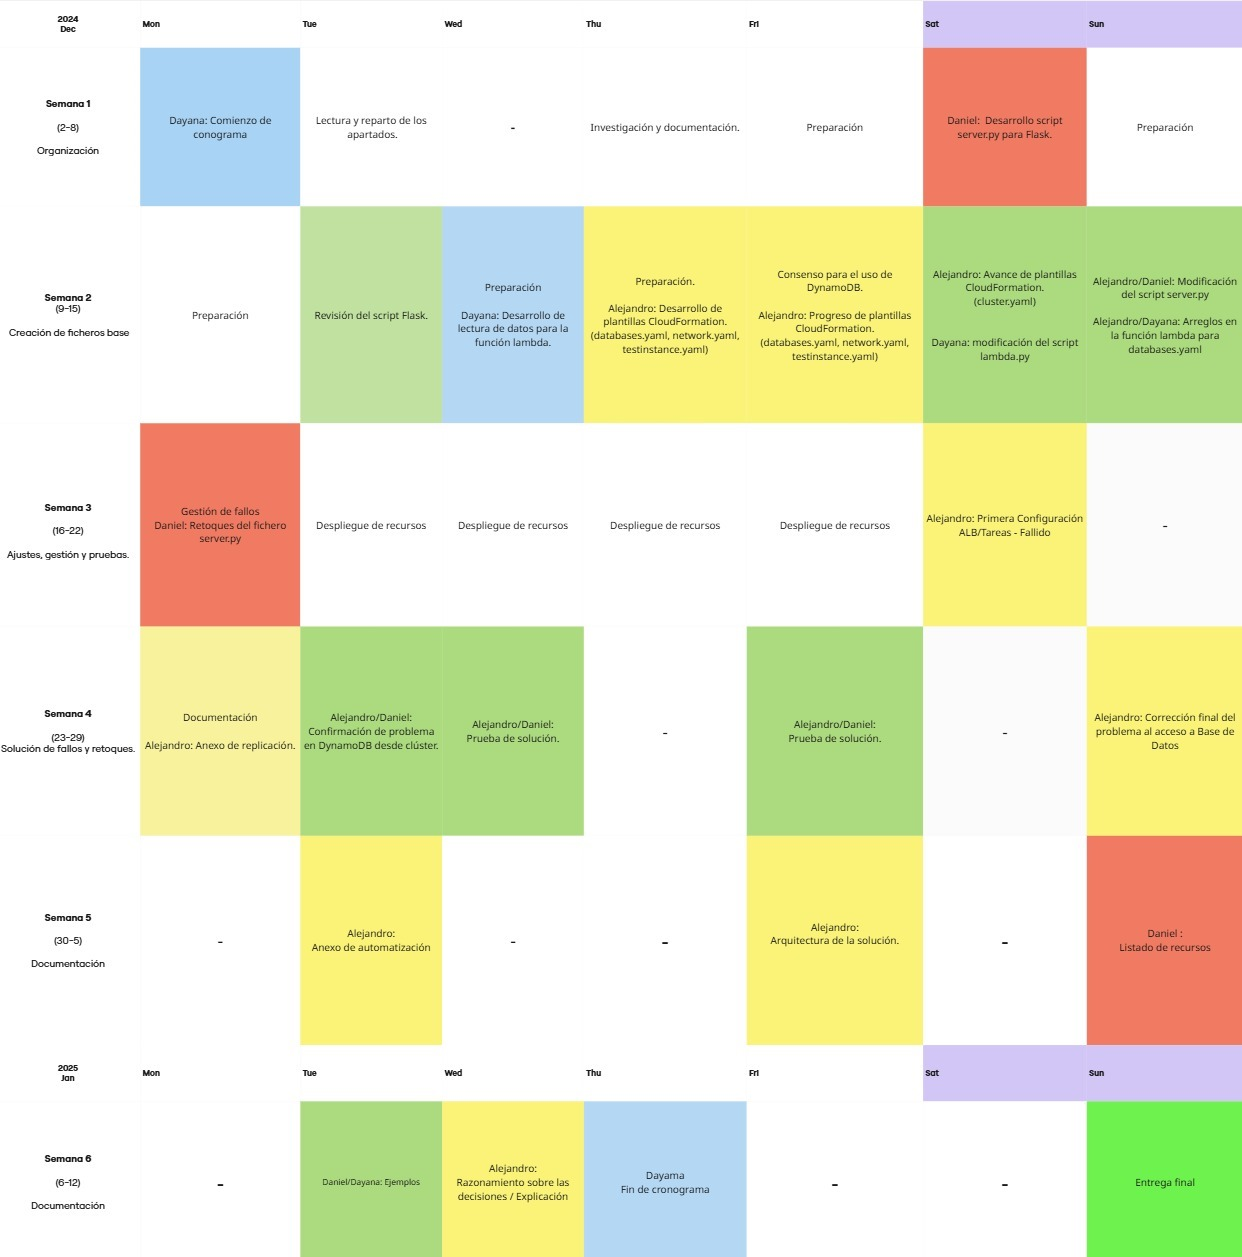
\includegraphics[width=\textwidth]{img/cronograma.jpeg}
\end{center}


\section{Arquitectura de la solución}

\includesvg[width=\textwidth]{img/diagrama.drawio.svg}


\section{Razonamiento sobre las decisiones de diseño}

\begin{itemize}
    \item \underline{\textit{Bucket S3 y Lambda}}. El \textit{bucket S3} es nuestra elección para la subida de datos gracias a su sencilla GUI y a su capacidad de crear una función \textit{Lambda} que se encargara de manejar los datos subidos en el mismo momento de subida de los datos.

    \item \underline{\textit{DynamoDB}} fue la base de datos seleccionada. Al principio pensamos que una base de datos SQL sería lo más sencillo, pero la escalabilidad de \textit{DynamoDB} fue lo que primero nos llamó la atención. Seguidamente, al investigarla, llegamos a la conclusión de que con una buena elección de claves (partición y ordenación), conseguiríamos no tener que preocuparnos de datos duplicados (explicación en la sección ``\textit{Pasos seguidos para la implementación y automatización}'').

    \item \underline{SNS} para el manejo de alertas por su sencilla implementación con \textit{boto3}.

    \item \underline{Una VPC} donde poder alojar las subredes públicas.

    \item \underline{Tres subredes públicas} para que el ALB tenga asegurado que al menos una funcione si dos fallan.

    \item \underline{Tres subredes privadas} para que si dos se caen, al menos una funcione.

    \item \underline{Un grupo de seguridad para el ALB} que solo acepte peticiones HTTP porque es lo único que queremos que acepte.

    \item \underline{Un grupo de seguridad para las instancias \textit{ECS}} que solo acepte peticiones HTTP del ALB porque es lo único que queremos que acepte.

    \item \underline{Una instancia para crear el contenedor} porque es la manera más ``automática'' de hacerlo.

    \item \underline{\textit{ECR}} para la imagen Docker que contiene el servidor web porque no tenemos más microservicios y con una imagen \textit{Docker} tenemos suficiente.

    \begin{itemize}
        \item Para la implementación del servidor web usamos \textit{Flask} y el \textit{SDK boto3} para el acceso al servicio \textit{DynamoDB}. 

        En todos los endpoints se usan los mismos argumentos ``year'' y ``month'' que se combinan para hacer una petición a la base de datos, esta petición se realiza con ``KeyConditionExpression'' porque al utilizarse la clave de particion es más rápido.
    \end{itemize}

    \item \underline{Clúster \textit{ECS}} para obtener una colección de instancias en distintas zonas de disponibilidad.

    \item \underline{ALB} para balancear la carga sobre las instancias \textit{ECS}.

    \item \underline{NAT GW} para que el servidor web tenga acceso a la base de datos.

    \item \underline{Combinación servicio/tarea} porque es una manera sencilla y muy configurable de arrancar el servidor web en las instancias.

    \item \underline{CloudFormation} y no AWS CLI porque es lo más sencillo de utilizar y la interfaz gráfica es muy intuitiva.
\end{itemize}


% \section{Servidor Web}

\subsection{server.py}
Para la implementación del servidor web usamos Flask y el SDK boto3 para el acceso al servicio DynamoDB. 

En todos los endpoints se usan los mismos argumentos 'year' y 'month' que se combinan para hacer una petición a la base de datos, esta petición se realiza con "KeyConditionExpression" porque al utilizarse la clave de particion es más rápido.

\begin{minted}[frame=single, linenos, breaklines]{python}
#!/usr/bin/env python3

import boto3
from flask import Flask, jsonify, request
from boto3.dynamodb.conditions import Key
import statistics

app = Flask(__name__)

# Conection to the DynamoBD resource and getting the corresponding table
dynamodb = boto3.resource('dynamodb', region_name='us-east-1')
table = dynamodb.Table('proy-stats')

# Gets the arguments of the request
def get_yearmonth():
    month, year = request.args.get('month'), request.args.get('year')
    try:
        month = int(month)
        year = int(year)
    except (ValueError, TypeError):
        return None
    return year * 100 + month

def build_json_response(dict_response, status):
    return jsonify(dict_response), status, {'Content-Type': 'application/json'}

# Default response for a well built request
def build_ok_json_response(dict_response):
    return build_json_response(dict_response, 200)

# Default response for a request with bad arguments
def get_invalid_args_response():
    http_code = 400  # Bad Request
    response_json = {
        'error': 'Invalid arguments. Make sure \'month\' and \'year\' are provided and are valid.'
    }
    return build_json_response(response_json, http_code)

# Response for a combination of month and year not found in DB.
def get_not_found_response():
    http_code = 404  # Not Found
    response_json = {
        'error': 'Combination of month and year not found in DB.'
    }
    return build_json_response(response_json, http_code)

# maxdiff endpoint
@app.route('/maxdiff')
def maxdiff():
    yearmonth = get_yearmonth()

    if yearmonth is None:
        return get_invalid_args_response()

    response = table.query(
        KeyConditionExpression=Key('YearMonth').eq(yearmonth)
    )

    items = response.get('Items', [])

    if len(items) == 0:
        return get_not_found_response()

    temperatures_mean = [t['Mean'] for t in items]
    result = {
        'result': max(temperatures_mean) - min(temperatures_mean)
    }
    return build_ok_json_response(result)

# sd endpoint
@app.route('/sd')
def sd():
    yearmonth = get_yearmonth()

    if yearmonth is None:
        return get_invalid_args_response()

    response = table.query(
        KeyConditionExpression=Key('YearMonth').eq(yearmonth)
    )

    items = response.get('Items', [])

    if len(items) == 0:
        return get_not_found_response()
    
    temperatures_deviation = [t['Deviation'] for t in items]
    result = {
        'result': max(temperatures_deviation)
    }
    return build_ok_json_response(result)

# temp endpoint
@app.route('/temp')
def temp():
    yearmonth = get_yearmonth()

    if yearmonth is None:
        return get_invalid_args_response()

    response = table.query(
        KeyConditionExpression=Key('YearMonth').eq(yearmonth)
    )

    items = response.get('Items', [])

    if len(items) == 0:
        return get_not_found_response()

    temperatures_mean = [t['Mean'] for t in items]
    result = {
        'result': statistics.mean(temperatures_mean)
    }
    return build_ok_json_response(result)

# endpoint to indicate to aws that all is well
@app.route('/health')
def health():
    result = {
      'status': 'UP',
      'message': 'Service is healthy'
    }
    return build_ok_json_response(result)

# Not valid URI
@app.errorhandler(404)
def page_not_found(_):
    http_code = 404  # Not Found
    response_json = {
        'error': 'URI is not valid. Options: /maxdiff , /sd , /temp'
    }
    return build_json_response(response_json, http_code)

if __name__ == '__main__':
    app.run(debug=True, host='0.0.0.0', port=80)


\end{minted}

\section{Recursos}

\begin{itemize}
    \item \underline{proy-landing-\$\{AWS::AccountId\}-\$\{AWS::Region\}}: Bucket S3 para la ingesta de datos. A él se sube un fichero CSV.

    \item \underline{proy-lambda}: Función \textit{Lambda} que parsea un CSV introducido en el bucket S3 e introduce los datos extraidos a una tabla de \textit{DynamoDB}.

    \item \underline{proy-stats}: Tabla de \textit{DynamoDB}. Aquí se guardan los datos que serán solicitados por el web server. Además, hemos optado por esta opción porque es un PaaS, por tanto no hay que preocuparse del escalado y será tolerante a fallos.

    \item \underline{proy-sns}: Tópico SNS. Notificación a través de email en el momento de la ingesta de datos si la desviación semanal supera $0.5$.

    \item \underline{proy-vpc}: VPC. Contiene toda la infraestructura de red necesaria para el correcto despliegue de la solución.

    \item \underline{proy-igw}: IGW. Ofrece conexión a internet para los servicios de \textit{proy-vpc} que lo requieran.

    \item \underline{proy-prt}: Tabla de enrutamiento que ofrece conexión a internet.

    \item \underline{proy-nat}: NAT GW. Ofrece conexión a internet a las instancias ECS que se encuentran en subredes privadas.

    \item \underline{proy-privateroutetable}: Tabla de enrutamiento que ofrece conexión a \textit{proy-nat}.

    \item \underline{proy-public-subnet-\{1, 2, 3\}}: Subredes públicas, cada una en una zona de disponibilidad diferente. Dan soporte a \textit{proy-nat}, a la instancia que crea la imagen \textit{Docker} y al ALB.

    \item \underline{proy-private-subnet-\{1, 2, 3\}}: Subredes privadas, cada una en una zona de disponibilidad diferente. Dan soporte a las instancias del clúster ECS.

    \item \underline{proy-BalancerSecurityGroup}: Grupo de seguridad que acepta peticiones HTTP en el puerto por defecto. Lo usa el ALB.

    \item \underline{proy-TaskSecurityGroup}: Grupo de seguridad que acepta peticiones HTTP en el puerto por defecto cuando vienen de ALB. Lo usan los servicios ECS y las instancias del clúster ECS.

    \item \underline{proyrepo}: Repositorio ECR que almacena la imagen \textit{Docker}.

    \item \underline{proy-TestInstance}: Instancia EC2. La usamos únicamente para crear el contenedor y subirlo a \textit{proyrepo}.

    \item \underline{proy-ECSLaunchTemplate}: Plantilla de lanzamiento. Usada para el correcto despliegue del clúster ECS.

    \item \underline{proy-cluster-ECSAutoScalingGroup-ID}: Grupo de autoescalado. Usado para el correcto despliegue del clúster ECS.

    \item \underline{proy-cluster-EC2CapacityProvider-ID}: Proveedor de capacidad. Usado para el correcto despliegue del clúster ECS.

    \item \underline{proy-cluster}: Clúster ECS. Utilizado para desplegar instancias ECS en tres subredes privadas (por seguridad), cada una en diferentes zonas de disponibilidad, y para aportar escalabilidad y tolerancia a fallos.

    \item \underline{proy-task}: Definición de Tarea ECS. Define la tarea de la cual se implementarán los servicios ECS.

    \item \underline{proy-cluster-ECSService-ID}: Servicios ECS. Implementaciones de \textit{proy-task}.

    \item \underline{proy-dest-grp}: Grupo de destino. Se encarga de proporcionar instancias al ALB.

    \item \underline{proy-alb}: Application Load Balancer. Usado para distribuir las peticiones entre las distintas tareas del cluster. Está en tres subredes públicas, cada una en una zona de disponibilidad, para tolerancia a fallos.

    \item \underline{proy-databases, proy-network, proy-testinstance, proy-cluster}: Pilas de CloudFormation. Se encargan de desplegar todo.

    \item \underline{Salidas de proy-network}: Utilizadas en otras pilas.
    \begin{itemize}
        \item ALBSGId: ID de \textit{proy-BalancerSecurityGroup}.
        \item TaskSGId: ID de \textit{proy-TaskSecurityGroup}.
        \item PrivateSubnet\{1, 2, 3\}: IDs de las subredes privadas.
        \item PublicSubnet\{1, 2, 3\}: IDs de las subredes públicas.
        \item VPCID: ID de la VPC.
    \end{itemize}

    \item \underline{ALBDNSName}: Salida de \textit{proy-cluster}. Utilizada para una fácil obtención del DNS del ALB.
\end{itemize}


\section{Pasos seguidos para la implementación y automatización}

Lo primero que se pensó es en cómo iba a funcionar el servidor web. Originalmente la aplicación que se encargaría del servidor solo iba a tener los tres endpoints que se piden en el enunciado, así que esos fueron los implementados. Sin controlar qué ocurriría con paths que no existen ni nada por el estilo. Además, no teníamos claro cómo iba a funcionar la tabla de \textit{DynamoDB}, así que se dejó un código de ``placeholder'' para la petición a la base de datos.

Una vez que teníamos una primera idea de cómo funcionaría el servidor, nos pusimos a planear cómo funcionaría la tabla de \textit{DynamoDB} con detalle. Tras un intercambio de ideas, llegamos a la conclusión de que subiríamos los datos con la siguiente estructura:

\begin{itemize}
    \item \underline{Clave de partición}: \texttt{YearMonth}. Este campo es el resultado de sumar el año multiplicado por cien al mes. De esta manera solo accedemos a una partición por consulta.
    \item \underline{Clave de ordenación}: \texttt{Day}. Este campo es el resultado de extraer el día de la columna ``Fecha'' del CSV. Con la combinación de esta clave de ordenación y la de partición hemos conseguido facilitar la tarea de evitar fechas duplicadas en la tabla de \textit{DynamoDB}, pues solo puede haber una combinación de valores al mismo tiempo y la que se queda es la última que se sube (tal y como se pide en el enunciado).
    \item \underline{Otros campos}: \texttt{Mean} y \texttt{Deviation}. Los campos que contienen los datos.
\end{itemize}

Con esto en mente se creó una plantilla de \textit{CloudFormation} que se encarga de crear la tabla, un \textit{Bucket S3} donde subir los CSVs, la función \textit{Lambda} y los permisos necesarios para que todos los servicios puedan comunicarse entre ellos. Además, nos pusimos a trabajar en los detalles del servidor web y de la función \textit{Lambda}. Los cambios al servidor web fueron sencillos, lo que más cambió es la resolución de errores. Con respecto a la función \textit{Lambda}, lo que primero se implementó es el correcto parseo de los datos y la correcta subida de los datos a la tabla de \textit{DynamoDB}. Gracias a nuestra elección de claves, el script solo tenía que encargarse de poner los datos en la tabla, sin preocuparse del contenido de la tabla.

Una vez todo el tema de la base de datos estaba solucionado, implementamos en la función \textit{Lambda} el sistema de alertas con el servicio \textit{SNS}, dando por finalizada la función y la plantilla mencionada anteriormente.

A continuación nos pusimos a crear una plantilla de \textit{CloudFormation} que se encargara de crear la arquitectura de la red y los grupos de seguridad, aunque también se encarga de crear el repositorio \textit{ECR} que contendría la imagen de Docker con el servidor web (más sobre esto más adelante). La red al principio contenía tres subredes públicas y ninguna privada, pues pensábamos proteger las instancias del clúster \textit{ECS} con un grupo de seguridad. Junto con las tres subredes se crearon tres grupos de seguridad:

\begin{itemize}
    \item Un grupo de seguridad para el balanceador de carga, que se encarga de aceptar las peticiones HTTP.
    \item Un grupo de seguridad para las instancias del clúster \textit{ECS}, que se encarga de aceptar las peticiones HTTP procedentes del balanceador de carga.
    \item Un grupo de seguridad para una instancia \textit{EC2} que se crearía en otra plantilla. Se encarga de aceptar peticiones HTTP y SSH.
\end{itemize}

Seguidamente nos pusimos a trabajar en la instancia de prueba y en su plantilla de \textit{CloudFormation}. Esta instancia se encarga de crear la imagen docker que contiene el servidor web, de subirla al repositorio \textit{ECR}, y de ejecutarla. Uno de nosotros ya hizo algo similar en una entrega de la asignatura, así que fue sencillo adaptarlo para esta implementación. La función Lambda ya sabíamos que funcionaba bien, pero con esta instancia de prueba pudimos comprobar y arreglar el servidor web de una manera sencilla.

Lo siguiente era la combinación de clúster, servicio/tareas y ALB. La implementación de todo fue bastante fluida, lo único que merece la pena nombrar es que como cualquier \textit{path} que no fuese uno de los tres del enunciado devuelve un error HTTP 404, el servicio no aparecía como desplegado nunca. Para solucionarlo, añadimos un nuevo endpoint (\textit{/health}).

Sin embargo, nos encontramos con un error que tratamos varios días de solucionar y es que, por alguna razón, las instancias no eran capaces de conectarse a la base de datos. Tras muchos intentos para solucionarlo, decidimos abandonar esta estructura de red y probar con otra. Los dos cambios fue la creación de tres subredes privadas que alojarían a las instancias \textit{ECS} y la creación de un GW NAT en una de las subredes públicas para darles acceso a la base de datos. Con estos cambios se solucionó el problema.

Una vez lo teníamos todo listo, hicimos una limpieza de las plantillas de \textit{CloudFormation}, eliminando el grupo de seguridad para la instancia \textit{EC2} de prueba y eliminando la línea que se encargaba de ejecutar la imagen de \textit{Docker} en esa instancia de pruebas.


\section{Ejemplos de la correcta ejecución}

\subsection{Ingesta de datos (Lambda)}

\begin{center}
     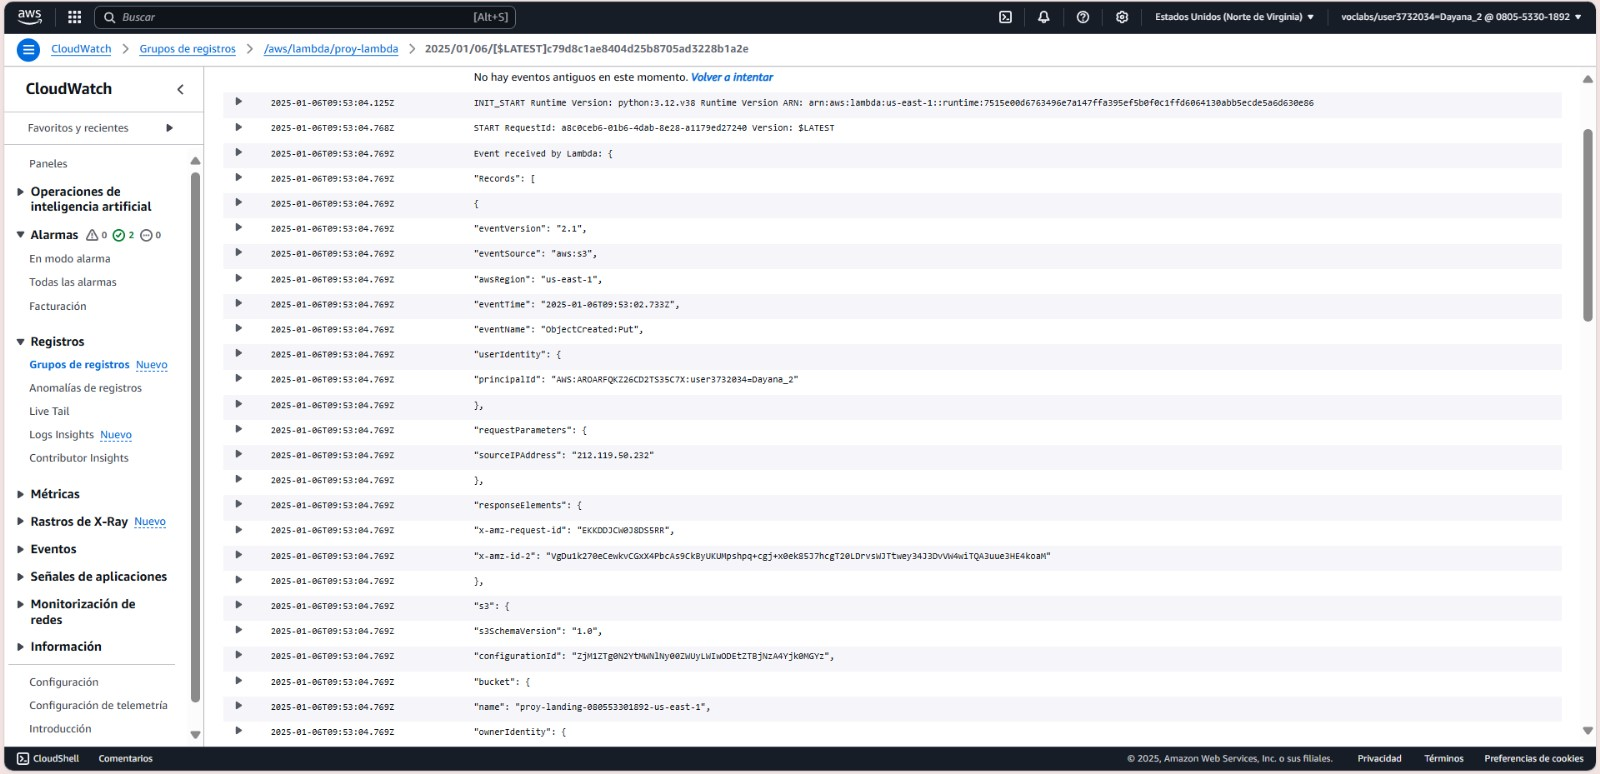
\includegraphics[width=0.5\textwidth]{img/ingesta1.jpeg}
     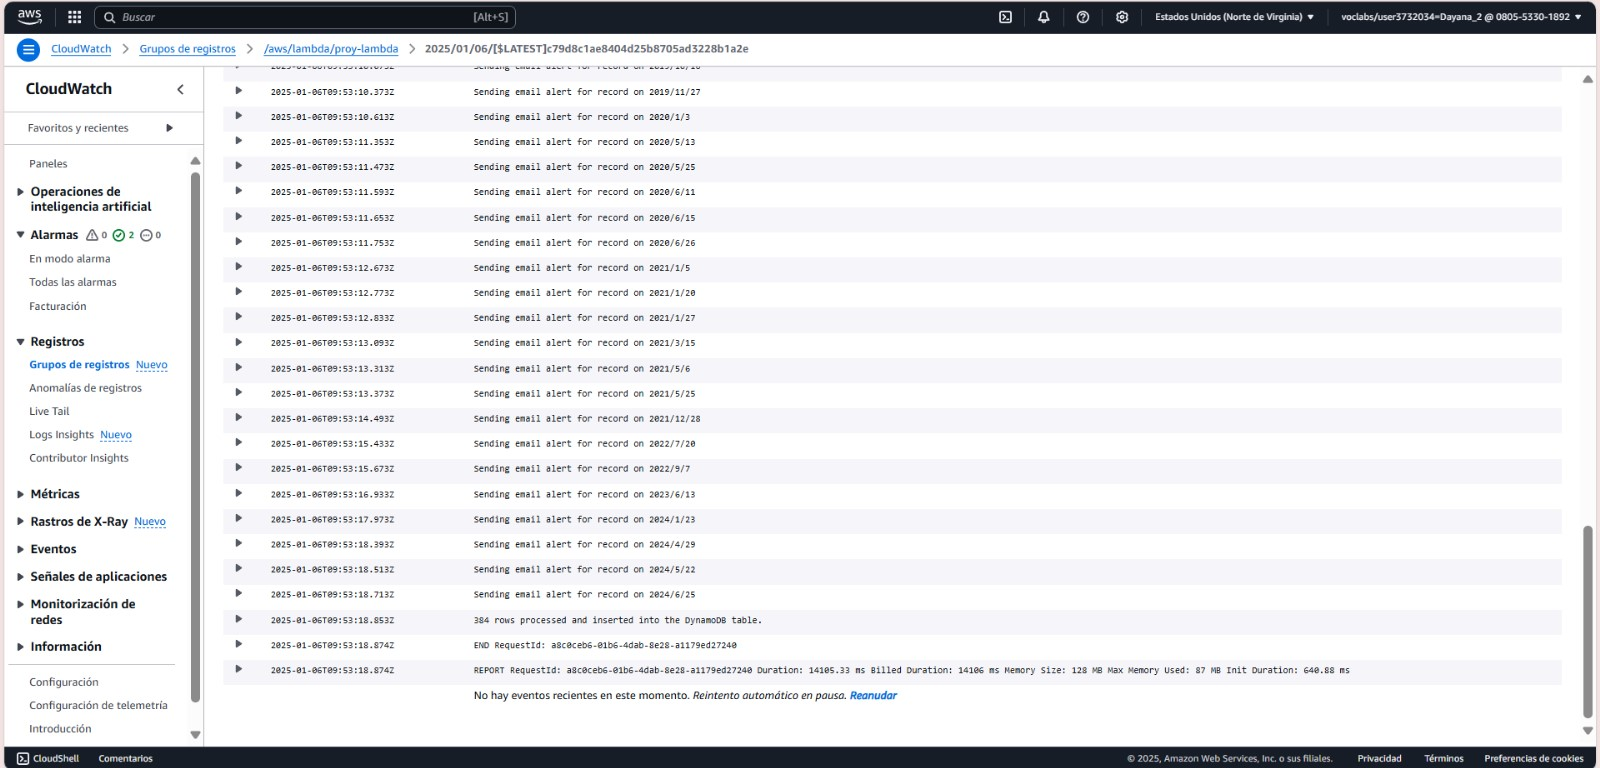
\includegraphics[width=0.5\textwidth]{img/ingesta2.jpeg}
\end{center}

\subsection{Alerta}

\begin{center}
     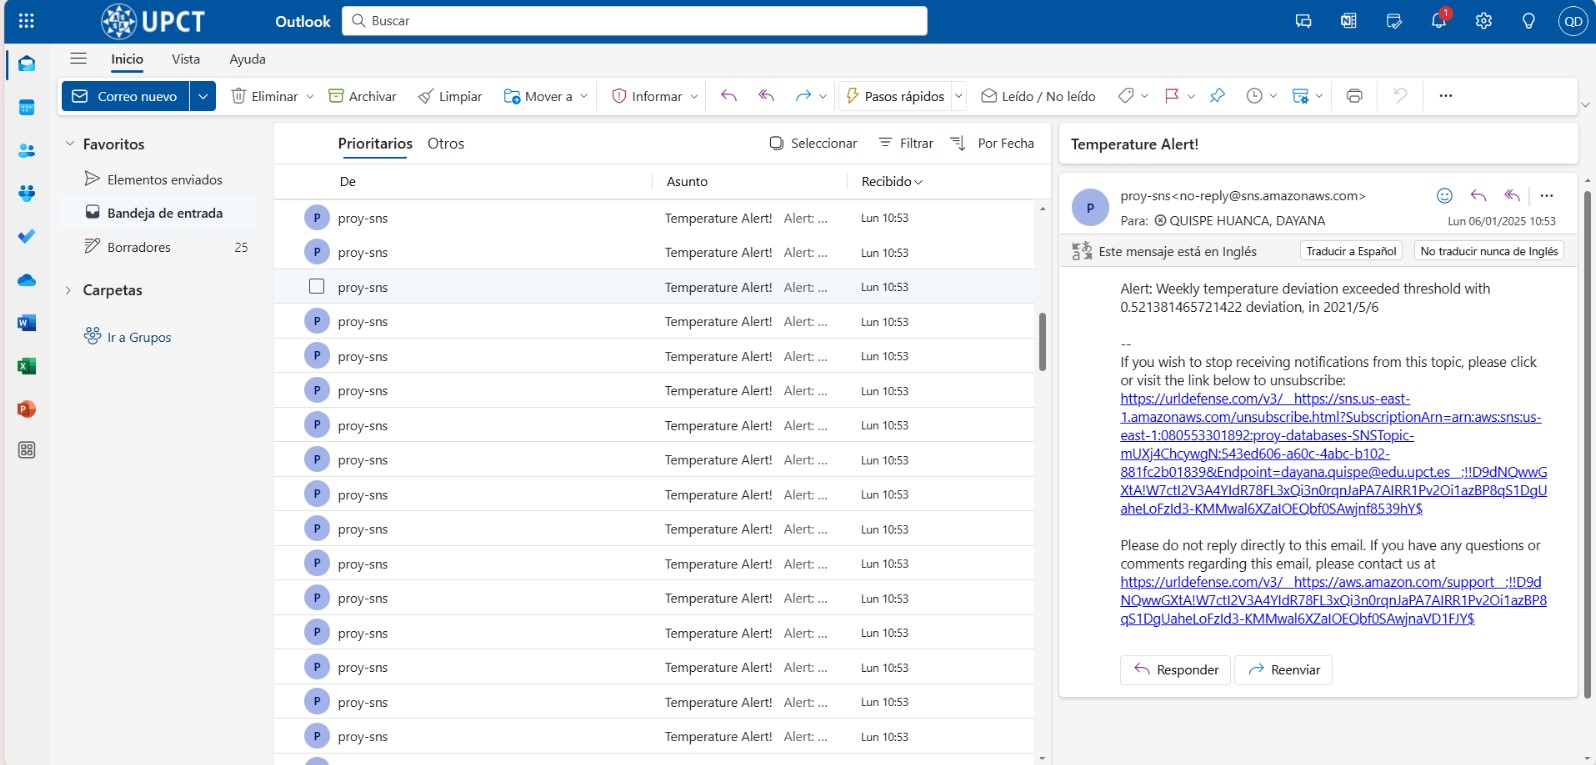
\includegraphics[width=0.5\textwidth]{img/alerta.jpeg}
\end{center}

\subsection{Peticiones web server}

\begin{center}
     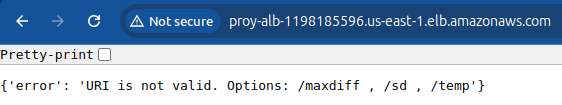
\includegraphics[width=0.5\textwidth]{img/noURI.png}
     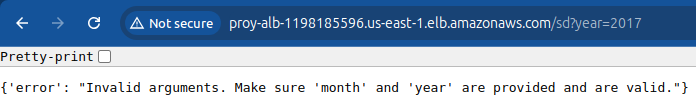
\includegraphics[width=0.5\textwidth]{img/notValidArguments.png}
     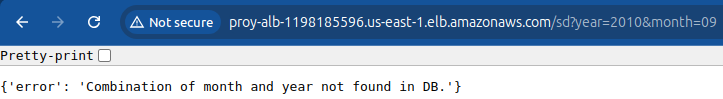
\includegraphics[width=0.5\textwidth]{img/dataNotFound.png}
     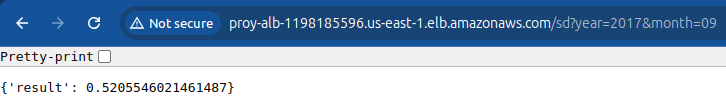
\includegraphics[width=0.5\textwidth]{img/validArguments.png}
\end{center}

\section{Anexo 1: Replicación}

Todo se despliega a través de CloudFormation, haciendo uso de su sistema de parámetros y salidas. Además, todas las pilas se llamarán igual que el fichero de la plantilla, sin la extensión \texttt{.yaml} y con el prefijo \texttt{proy-}. Para cada plantilla hay que configurar el rol de IAM como \textit{LabRole}.

\subsection{proy-databases}

El primer fichero que se sube se llama \texttt{databases.yaml}. Este fichero se encarga de crear el bucket que recibe los ficheros, la función Lambda que procesa dichos ficheros, la tabla de \textit{DynamoDB} y el tópico de \textit{SNS}. Los dos parámetros que necesita son:

\begin{itemize}
     \item \underline{IAMRoleName}: Nombre del rol que se asociará a la función Lambda.
     \item \underline{EmailTarget}: Correo al que se enviará una alerta cuando se encuentre una desviación mayor a $0.5$.
\end{itemize}

Se recomienda dejar \textit{IAMRoleName} con su valor por defecto, mientras que el email se puede configurar como se guste (mientras sea válido).

No hace falta esperar a que esta plantilla termine para continuar, pues esta plantilla es completamente independiente al resto.

\subsection{proy-network}

El segundo fichero es \texttt{network.yaml}. Esta plantilla se encarga de crear la infraestructura de red que dará soporte a las instancias EC2. En concreto:

\begin{itemize}
    \item VPC.
    \item Internet Gateway.
    \item Tabla de enrutamiento con acceso a internet.
    \item Tabla de enrutamiento para las subredes privadas.
    \item Tres subredes públicas, cada una en una zona distinta.
    \item Tres subredes privadas, cada una en una zona distinta.
    \item Un GW NAT.
    \item Dos grupos de seguridad, uno para el balanceador de carga y otro para las instancias EC2 y la tarea.
    \item El repositorio ECR que contendrá el contenedor Docker (creado en el siguiente paso).
    \item Todo lo necesario para que todo lo anterior se despliegue adecuadamente.
\end{itemize}

Esta plantilla no tiene parámetros, pero sí que tiene salidas. Las salidas son los IDs de la VPC, las subredes, y de los grupos de seguridad.

Los siguientes pasos necesitan del funcionamiento de esta pila.

\subsection{proy-testinstance}

El tercer fichero es \texttt{testinstance.yaml}. Esta plantilla se encarga de crear una instancia que construirá el contenedor Docker y la subirá al contenedor creado en la plantilla anterior. La plantilla necesita tres parámetros:

\begin{itemize}
    \item \underline{ECRPassword}: Contraseña utilizada para el acceso a ECR. Normalmente sigue la estructura siguiente:
    \begin{itemize}
        \item \texttt{ACCOUNTID.dkr.ecr.REGION.amazonaws.com} (lo que habría que cambiar son los doce dígitos del principio).
    \end{itemize}
    \item \underline{ECRUsername}: Igual para todos, así que no habría que cambiarlo. Se ha dejado como parámetro por si esto lo cambian en el futuro.
    \item \underline{IAMProfile}: Perfil IAM para la instancia. El valor por defecto es válido.
\end{itemize}

Una vez que sea seguro que el contenedor está subido, esta pila se puede eliminar, pues ya habría cumplido su propósito y no se necesita su existencia de aquí en adelante. Eso sí, no continuar con el último paso hasta que el contenedor se haya subido, pues es necesario.

\subsection{proy-cluster}

El cuarto y último fichero es \texttt{cluster.yaml}. Esta plantilla se encarga de crear la tarea, los servicios, el balanceador de carga y el cluster ECS. Los parámetros se deben dejar por defecto (a no ser de que se sepa lo que se está haciendo).

\begin{itemize}
    \item \underline{LatestECSOptimizedAMI}: ID de una AMI válida.
    \item \underline{IAMProfile}: Perfil IAM usado para la plantilla de despliegue del clúster.
    \item \underline{IAMRoleName}: Nombre del rol IAM usado en la definición de la tarea.
\end{itemize}

Tarda un poco en desplegarse, pero cuando termine ya se habrá terminado de crear todo lo necesario para le entrega.


\section{Anexo 2: Automatización}

\subsection{databases.yaml}

\begin{minted}[frame=single, linenos, breaklines]{yaml}
AWSTemplateFormatVersion: 2010-09-09
Description: >-
  Creates the neccesary bucket, lambda function, DynamoDB table, and SNS topic.

####################
# Parameters section
####################

Parameters:
  IAMRoleName:
    Description: IAM role used for the lambda function
    Type: String
    Default: LabRole

  EmailTarget:
    Description: Email addresss used by SNS
    Type: String
    Default: email@host.com

###################
# Resources section
###################

Resources:

  ## Bucket

  LandingZoneBucket:
    Type: AWS::S3::Bucket
    DependsOn: LambdaPermission
    Properties:
      BucketName: !Sub proy-landing-${AWS::AccountId}-${AWS::Region}
      NotificationConfiguration:
        LambdaConfigurations:
          - Event: s3:ObjectCreated:*
            Function: !GetAtt LambdaFunction.Arn

  BucketPolicy:
    Type: AWS::S3::BucketPolicy
    DependsOn: LandingZoneBucket
    Properties:
      Bucket: !Ref LandingZoneBucket
      PolicyDocument:
        Version: 2012-10-17
        Statement:
          - Effect: Allow
            Principal:
              Service: lambda.amazonaws.com
            Action:
              - "s3:GetObject"
            Resource: !Sub "arn:aws:s3:::${LandingZoneBucket}/*"

  ## Lambda

  LambdaFunction:
    Type: AWS::Lambda::Function
    Properties:
      FunctionName: proy-lambda
      Handler: index.lambda_handler
      Runtime: python3.12
      Timeout: 300
      Role: !Sub arn:aws:iam::${AWS::AccountId}:role/${IAMRoleName}
      Code:
        ZipFile: |
          import json, urllib, boto3, csv
          from datetime import datetime
          from decimal import Decimal

          # Connect to AWS S3 and DynamoDB
          s3 = boto3.resource('s3')
          dynamodb = boto3.resource('dynamodb', region_name='us-east-1')

          # Connect to SNS 
          sns = boto3.client('sns') 
          stack_name = 'proy-databases' 
          snsTopicArn = [t['TopicArn'] for t in sns.list_topics()['Topics'] 
                          if stack_name in t['TopicArn']][0] 

          # Connect to the DynamoDB table
          stats_table = dynamodb.Table('proy-stats')

          def lambda_handler(event, context):
              # Show the incoming event in the debug log 
              print('Event received by Lambda: ' + json.dumps(event, indent=2))

              # Extract the bucket name and object key from the event
              bucket = event['Records'][0]['s3']['bucket']['name']
              key = urllib.parse.unquote_plus(event['Records'][0]['s3']['object']['key'])
              local_filename = '/tmp/stats.csv'

              # Download the file from S3 to the local filesystem
              try:
                  s3.meta.client.download_file(bucket, key, local_filename)
              except Exception as e:
                  print(e)
                  print(f'Error retrieving object {key} from bucket {bucket}. Ensure it exists and is in the same region as this function.')
                  raise e

              # Process the CSV file
              row_count = 0
              try:
                  with open(local_filename, 'r') as csvfile:
                      reader = csv.DictReader(csvfile, delimiter=',')
                      for row in reader:
                          row_count += 1

                          #Validate and process each row
                          try:
                              date_str = row['Fecha']
                              mean = Decimal(row['Medias'])
                              deviation = Decimal(row['Desviaciones'])

                              if deviation > 0.5:
                                  #Message:
                                  message = (f"Alert: Weekly temperature deviation exceeded threshold with {deviation} deviation, in {date_str}")
                                  
                                  print(f"Sending email alert for record on {date_str}")

                                  # Send message to SNS 
                                  sns.publish( 
                                      TopicArn=snsTopicArn, 
                                      Message=message, 
                                      Subject='Temperature Alert!', 
                                      MessageStructure='raw' 
                                  )

                              # Convert the date and calculate YearMonth and Day
                              date_obj = datetime.strptime(date_str, '%Y/%m/%d')
                              year_month = 100 * date_obj.year + date_obj.month
                              day = date_obj.day

                              # Insert into the DynamoDB table
                              stats_table.put_item(
                                  Item={
                                      'YearMonth': year_month,
                                      'Day': day,
                                      'Mean': mean,
                                      'Deviation': deviation
                                  }
                              )
                          except Exception as e:
                              print(f'Error processing row: {row}. Details: {e}')

              except Exception as e:
                  print(f'Error reading or processing the CSV file: {e}')
                  raise e

              # Finished
              print(f'{row_count} rows processed and inserted into the DynamoDB table.')

  LambdaPermission:
    Type: AWS::Lambda::Permission
    Properties:
      FunctionName: !GetAtt LambdaFunction.Arn
      Action: lambda:InvokeFunction
      Principal: s3.amazonaws.com
      SourceAccount: !Ref AWS::AccountId

  ## DynamoDB

  # YearMonth | Day | Mean | Deviation
  #
  # YearMonth = 100 * Year + Month

  DynamoTable:
    Type: AWS::DynamoDB::Table
    Properties:
      TableName: proy-stats
      AttributeDefinitions:
        - AttributeName: YearMonth
          AttributeType: N
        - AttributeName: Day
          AttributeType: N
      KeySchema:
        - AttributeName: YearMonth
          KeyType: HASH   # Partition Key
        - AttributeName: Day
          KeyType: RANGE  # Sort Key
      BillingMode: PAY_PER_REQUEST

  # SNS

  SNSTopic:
    Type: AWS::SNS::Topic
    Properties:
      DisplayName: proy-sns
      Subscription:
        - Endpoint: !Ref EmailTarget
          Protocol: email
\end{minted}


\subsection{network.yaml}

\begin{minted}[frame=single, linenos, breaklines]{yaml}
AWSTemplateFormatVersion: 2010-09-09
Description: >-
  Creates the network's infraestructure and creates the ECR repo.

###################
# Resources section
###################

Resources:

  ## VPC

  VPC:
    Type: AWS::EC2::VPC
    Properties:
      CidrBlock: 192.168.0.0/16
      Tags:
        - Key: Name
          Value: proy-vpc

  ## Internet Gateway

  InternetGateway:
    Type: AWS::EC2::InternetGateway
    Properties:
      Tags:
        - Key: Name
          Value: proy-igw

  VPCGatewayAttachment:
    Type: AWS::EC2::VPCGatewayAttachment
    Properties:
      VpcId: !Ref VPC
      InternetGatewayId: !Ref InternetGateway

  ## Public Route Table

  PublicRouteTable:
    Type: AWS::EC2::RouteTable
    Properties:
      VpcId: !Ref VPC
      Tags:
        - Key: Name
          Value: proy-prt  # Public Route Table

  PublicRoute:
    Type: AWS::EC2::Route
    DependsOn: VPCGatewayAttachment
    Properties:
      RouteTableId: !Ref PublicRouteTable
      DestinationCidrBlock: 0.0.0.0/0
      GatewayId: !Ref InternetGateway

  ## NAT GW

  NatGatewayIP:
    Type: AWS::EC2::EIP
    DependsOn: VPCGatewayAttachment
    Properties:
      Domain: vpc

  NatGateway:
    Type: AWS::EC2::NatGateway
    Properties:
      AllocationId: !GetAtt NatGatewayIP.AllocationId
      SubnetId: !Ref PublicSubnet1
      Tags:
        - Key: Name
          Value: proy-nat

  ## Private Route Table

  PrivateRouteTable:
    Type: AWS::EC2::RouteTable
    Properties:
      VpcId: !Ref VPC
      Tags:
        - Key: Name
          Value: proy-privateroutetable

  DefaultPrivateRoute:
    Type: AWS::EC2::Route
    Properties:
      RouteTableId: !Ref PrivateRouteTable
      DestinationCidrBlock: 0.0.0.0/0
      NatGatewayId: !Ref NatGateway

  ## Public Subnet 1

  PublicSubnet1:
    Type: AWS::EC2::Subnet
    Properties:
      VpcId: !Ref VPC
      CidrBlock: 192.168.1.0/24
      AvailabilityZone: us-east-1a
      Tags:
        - Key: Name
          Value: proy-public-subnet-1

  PublicSubnetRouteTableAssociation1:
    Type: AWS::EC2::SubnetRouteTableAssociation
    Properties:
      SubnetId: !Ref PublicSubnet1
      RouteTableId: !Ref PublicRouteTable

  PublicSubnetNetworkAclAssociation1:
    Type: AWS::EC2::SubnetNetworkAclAssociation
    Properties:
      SubnetId: !Ref PublicSubnet1
      NetworkAclId: !GetAtt 
        - VPC
        - DefaultNetworkAcl

  ## Public Subnet 2

  PublicSubnet2:
    Type: AWS::EC2::Subnet
    Properties:
      VpcId: !Ref VPC
      CidrBlock: 192.168.2.0/24
      AvailabilityZone: us-east-1b
      Tags:
        - Key: Name
          Value: proy-public-subnet-2

  PublicSubnetRouteTableAssociation2:
    Type: AWS::EC2::SubnetRouteTableAssociation
    Properties:
      SubnetId: !Ref PublicSubnet2
      RouteTableId: !Ref PublicRouteTable

  PublicSubnetNetworkAclAssociation2:
    Type: AWS::EC2::SubnetNetworkAclAssociation
    Properties:
      SubnetId: !Ref PublicSubnet2
      NetworkAclId: !GetAtt 
        - VPC
        - DefaultNetworkAcl

  ## Public Subnet 3

  PublicSubnet3:
    Type: AWS::EC2::Subnet
    Properties:
      VpcId: !Ref VPC
      CidrBlock: 192.168.3.0/24
      AvailabilityZone: us-east-1c
      Tags:
        - Key: Name
          Value: proy-public-subnet-3

  PublicSubnetRouteTableAssociation3:
    Type: AWS::EC2::SubnetRouteTableAssociation
    Properties:
      SubnetId: !Ref PublicSubnet3
      RouteTableId: !Ref PublicRouteTable

  PublicSubnetNetworkAclAssociation3:
    Type: AWS::EC2::SubnetNetworkAclAssociation
    Properties:
      SubnetId: !Ref PublicSubnet3
      NetworkAclId: !GetAtt 
        - VPC
        - DefaultNetworkAcl

  ## Private Subnet 1

  PrivateSubnet1:
    Type: AWS::EC2::Subnet
    Properties:
      VpcId: !Ref VPC
      CidrBlock: 192.168.4.0/24
      AvailabilityZone: us-east-1a
      Tags:
        - Key: Name
          Value: proy-private-subnet-1

  PrivateSubnet1RouteTableAssociation:
    Type: AWS::EC2::SubnetRouteTableAssociation
    Properties:
      RouteTableId: !Ref PrivateRouteTable
      SubnetId: !Ref PrivateSubnet1

  ## Private Subnet 2

  PrivateSubnet2:
    Type: AWS::EC2::Subnet
    Properties:
      VpcId: !Ref VPC
      CidrBlock: 192.168.5.0/24
      AvailabilityZone: us-east-1b
      Tags:
        - Key: Name
          Value: proy-private-subnet-2

  PrivateSubnet2RouteTableAssociation:
    Type: AWS::EC2::SubnetRouteTableAssociation
    Properties:
      RouteTableId: !Ref PrivateRouteTable
      SubnetId: !Ref PrivateSubnet2

  ## Private Subnet 3

  PrivateSubnet3:
    Type: AWS::EC2::Subnet
    Properties:
      VpcId: !Ref VPC
      CidrBlock: 192.168.6.0/24
      AvailabilityZone: us-east-1c
      Tags:
        - Key: Name
          Value: proy-private-subnet-3

  PrivateSubnet3RouteTableAssociation:
    Type: AWS::EC2::SubnetRouteTableAssociation
    Properties:
      RouteTableId: !Ref PrivateRouteTable
      SubnetId: !Ref PrivateSubnet3

  ## Security Groups

  SecurityGroupBalancer:
    Type: AWS::EC2::SecurityGroup
    Properties:
      GroupDescription: Allow HTTP Ingress
      GroupName: proy-BalancerSecurityGroup
      SecurityGroupIngress:
        - IpProtocol: tcp
          FromPort: 80
          ToPort: 80
          CidrIp: 0.0.0.0/0
      VpcId: !Ref VPC

  SecurityGroupTask:
    Type: AWS::EC2::SecurityGroup
    Properties:
      GroupDescription: Allow HTTP Ingress from proy-BalancerSecurityGroup
      GroupName: proy-TaskSecurityGroup
      SecurityGroupIngress:
        - IpProtocol: tcp
          FromPort: 80
          ToPort: 80
          SourceSecurityGroupId: !Ref SecurityGroupBalancer
      VpcId: !Ref VPC

  ## Container Registry

  ECRRepo:
    Type: AWS::ECR::Repository
    Properties:
      RepositoryName: proyrepo

###################
# Resources section
###################

Outputs:
  VPCId:
    Description: VPC ID
    Value: !Ref VPC
    Export:
      Name: proy-VPCId

  PublicSubnet1Id:
    Description: Public Subnet 1 ID
    Value: !Ref PublicSubnet1
    Export:
      Name: proy-PublicSubnet1Id

  PublicSubnet2Id:
    Description: Public Subnet 2 ID
    Value: !Ref PublicSubnet2
    Export:
      Name: proy-PublicSubnet2Id

  PublicSubnet3Id:
    Description: Public Subnet 3 ID
    Value: !Ref PublicSubnet3
    Export:
      Name: proy-PublicSubnet3Id

  PrivateSubnet1Id:
    Description: Private Subnet 1 ID
    Value: !Ref PrivateSubnet1
    Export:
      Name: proy-PrivateSubnet1Id

  PrivateSubnet2Id:
    Description: Private Subnet 2 ID
    Value: !Ref PrivateSubnet2
    Export:
      Name: proy-PrivateSubnet2Id

  PrivateSubnet3Id:
    Description: Private Subnet 3 ID
    Value: !Ref PrivateSubnet3
    Export:
      Name: proy-PrivateSubnet3Id

  ALBSGId:
    Description: proy-BalancerSecurityGroup
    Value: !Ref SecurityGroupBalancer
    Export:
      Name: proy-ALBSGId

  TaskSGId:
    Description: proy-TaskSecurityGroup ID
    Value: !Ref SecurityGroupTask
    Export:
      Name: proy-TaskSGId
\end{minted}


\subsection{testinstance.yaml}

\begin{minted}[frame=single, linenos, breaklines]{yaml}
AWSTemplateFormatVersion: 2010-09-09
Description: >-
  Creates an instance that builds and uploads the Docker Container to the ECR.

####################
# Parameters section
####################

Parameters:
  IAMProfile:
    Description: PREVIOUSLY existing IAM Instance Profile
    Type: String
    Default: LabInstanceProfile

  ECRUsername:
    Description: Username used in ECR
    Type: String
    Default: AWS

  ECRPassword:
    Description: Password used in ECR
    Type: String
    Default: 592806013290.dkr.ecr.us-east-1.amazonaws.com

###################
# Resources section
###################

Resources:

  ## Instance

  Instance:
    Type: AWS::EC2::Instance
    Properties:
      InstanceType: t2.micro
      ImageId: ami-08a0d1e16fc3f61ea
      IamInstanceProfile: !Ref IAMProfile
      NetworkInterfaces:
        - AssociatePublicIpAddress: true
          DeviceIndex: 0
          DeleteOnTermination: true
          SubnetId: !ImportValue proy-PublicSubnet1Id
      Tags:
        - Key: Name
          Value: proy-TestInstance
      UserData:
        Fn::Base64: !Sub |
          #!/bin/bash

          dnf update -y
          dnf -y install docker
          sudo systemctl start docker
          sudo systemctl enable docker

          sudo echo "
          boto3
          Flask
          " > /etc/profile.d/requirements.txt

          sudo echo "
          #!/usr/bin/env python3

          import boto3
          from flask import Flask, jsonify, request
          from boto3.dynamodb.conditions import Key
          import statistics

          app = Flask(__name__)

          dynamodb = boto3.resource('dynamodb', region_name='us-east-1')
          table = dynamodb.Table('proy-stats')

          def get_yearmonth():
              month, year = request.args.get('month'), request.args.get('year')
              try:
                  month = int(month)
                  year = int(year)
              except (ValueError, TypeError):
                  return None
              return year * 100 + month

          def build_json_response(dict_response, status):
              return jsonify(dict_response), status, {'Content-Type': 'application/json'}

          def build_ok_json_response(dict_response):
              return build_json_response(dict_response, 200)

          def get_invalid_args_response():
              http_code = 400  # Bad Request
              response_json = {
                  'error': 'Invalid arguments. Make sure \'month\' and \'year\' are provided and are valid.'
              }
              return build_json_response(response_json, http_code)

          def get_not_found_response():
              http_code = 404  # Not Found
              response_json = {
                  'error': 'Combination of month and year not found in DB.'
              }
              return build_json_response(response_json, http_code)

          @app.route('/maxdiff')
          def maxdiff():
              yearmonth = get_yearmonth()

              if yearmonth is None:
                  return get_invalid_args_response()

              response = table.query(
                  KeyConditionExpression=Key('YearMonth').eq(yearmonth)
              )

              items = response.get('Items', [])

              if len(items) == 0:
                  return get_not_found_response()

              temperatures_mean = [t['Mean'] for t in items]
              result = {
                  'result': max(temperatures_mean) - min(temperatures_mean)
              }
              return build_ok_json_response(result)

          @app.route('/sd')
          def sd():
              yearmonth = get_yearmonth()

              if yearmonth is None:
                  return get_invalid_args_response()

              response = table.query(
                  KeyConditionExpression=Key('YearMonth').eq(yearmonth)
              )

              items = response.get('Items', [])

              if len(items) == 0:
                  return get_not_found_response()
              
              temperatures_deviation = [t['Deviation'] for t in items]
              result = {
                  'result': max(temperatures_deviation)
              }
              return build_ok_json_response(result)

          @app.route('/temp')
          def temp():
              yearmonth = get_yearmonth()

              if yearmonth is None:
                  return get_invalid_args_response()

              response = table.query(
                  KeyConditionExpression=Key('YearMonth').eq(yearmonth)
              )

              items = response.get('Items', [])

              if len(items) == 0:
                  return get_not_found_response()

              temperatures_mean = [t['Mean'] for t in items]
              result = {
                  'result': statistics.mean(temperatures_mean)
              }
              return build_ok_json_response(result)

          @app.route('/health')
          def health():
              result = {
                'status': 'UP',
                'message': 'Service is healthy'
              }
              return build_ok_json_response(result)

          @app.errorhandler(404)
          def page_not_found(_):
              http_code = 404  # Not Found
              response_json = {
                  'error': 'URI is not valid. Options: /maxdiff , /sd , /temp'
              }
              return build_json_response(response_json, http_code)


          if __name__ == '__main__':
              app.run(debug=True, host='0.0.0.0', port=80)
          " > /etc/profile.d/flask_app.py

          sudo echo "
          #syntax = docker/dockerfile:1.4
          FROM python:3.9-alpine
          WORKDIR /app
          COPY requirements.txt requirements.txt
          RUN pip3 install -r requirements.txt
          COPY flask_app.py flask_app.py
          CMD [\"python\", \"flask_app.py\"]
          " > /etc/profile.d/Dockerfile

          sudo docker build -t proy_flask_container /etc/profile.d/

          sudo aws ecr get-login-password --region us-east-1 | sudo docker login --username ${ECRUsername} --password-stdin ${ECRPassword}
          sudo docker tag proy_flask_container ${AWS::AccountId}.dkr.ecr.${AWS::Region}.amazonaws.com/proyrepo:proy_flask_container
          sudo docker push ${AWS::AccountId}.dkr.ecr.${AWS::Region}.amazonaws.com/proyrepo:proy_flask_container
\end{minted}


\subsection{cluster.yaml}

\begin{minted}[frame=single, linenos, breaklines]{yaml}
AWSTemplateFormatVersion: 2010-09-09
Description: >-
  Creates the ECS Cluster and the ALB.

####################
# Parameters section
####################

Parameters:

  LatestECSOptimizedAMI:
    Description: AMI ID
    Type: AWS::SSM::Parameter::Value<AWS::EC2::Image::Id>
    Default: /aws/service/ecs/optimized-ami/amazon-linux-2023/recommended/image_id

  IAMProfile:
    Description: PREVIOUSLY existing IAM Instance Profile
    Type: String
    Default: LabInstanceProfile

  IAMRoleName:
    Description: IAM role used for task execution
    Type: String
    Default: LabRole

###################
# Resources section
###################

Resources:

  ## Cluster

  ECSLaunchTemplate:
    Type: AWS::EC2::LaunchTemplate
    DependsOn: ECSCluster
    Properties:
      LaunchTemplateName: proy-ECSLaunchTemplate
      LaunchTemplateData:
        ImageId: !Ref LatestECSOptimizedAMI
        NetworkInterfaces:
          - AssociatePublicIpAddress: true
            DeviceIndex: 0
            DeleteOnTermination: true
            Groups: 
              - !ImportValue proy-TaskSGId
        InstanceType: t2.micro
        IamInstanceProfile:
          Arn: !Sub arn:aws:iam::${AWS::AccountId}:instance-profile/${IAMProfile}
        UserData: !Base64
          Fn::Sub:
            - |-
              #!/bin/bash
              echo ECS_CLUSTER=${ClusterName} >> /etc/ecs/ecs.config;
            - ClusterName: proy-cluster

  ECSAutoScalingGroup:
    Type: AWS::AutoScaling::AutoScalingGroup
    DependsOn: ECSCluster
    Properties:
      MinSize: 3
      MaxSize: 9
      DesiredCapacity: 3
      LaunchTemplate:
        LaunchTemplateId: !Ref ECSLaunchTemplate
        Version: !GetAtt ECSLaunchTemplate.LatestVersionNumber
      VPCZoneIdentifier:
        - !ImportValue proy-PrivateSubnet1Id
        - !ImportValue proy-PrivateSubnet2Id
        - !ImportValue proy-PrivateSubnet3Id
      Tags:
        - Key: Name
          PropagateAtLaunch: true
          Value: proy-cluster's ECS Instance

  ECSCluster:
    Type: AWS::ECS::Cluster
    Properties:
      ClusterName: proy-cluster
      ClusterSettings:
        - Name: containerInsights
          Value: disabled
      ServiceConnectDefaults:
        Namespace: proy-cluster
      Tags:
        - Key: cluster-ecs
          Value: proy

  EC2CapacityProvider:
    Type: AWS::ECS::CapacityProvider
    Properties:
      AutoScalingGroupProvider:
        AutoScalingGroupArn: !Ref ECSAutoScalingGroup
        ManagedScaling:
          Status: ENABLED
          TargetCapacity: 100
        ManagedTerminationProtection: DISABLED

  ClusterCPAssociation:
    Type: AWS::ECS::ClusterCapacityProviderAssociations
    DependsOn: ECSCluster
    Properties:
      Cluster: proy-cluster
      CapacityProviders:
        - !Ref EC2CapacityProvider
      DefaultCapacityProviderStrategy:
        - Base: 0
          Weight: 1
          CapacityProvider: !Ref EC2CapacityProvider

  ## Task

  TaskDefinition:
    Type: AWS::ECS::TaskDefinition
    Properties:
      Family: proy-task
      Cpu: 250
      Memory: 330
      NetworkMode: awsvpc
      TaskRoleArn: !Sub arn:aws:iam::${AWS::AccountId}:role/${IAMRoleName}
      ExecutionRoleArn: !Sub arn:aws:iam::${AWS::AccountId}:role/${IAMRoleName}
      ContainerDefinitions:
        - Name: proy_flask_container
          Image: !Sub ${AWS::AccountId}.dkr.ecr.${AWS::Region}.amazonaws.com/proyrepo:proy_flask_container
          Cpu: 250
          Memory: 330
          PortMappings:
            - ContainerPort: 80
              Protocol: tcp

  ## Service

  ECSService:
    Type: AWS::ECS::Service
    DependsOn:
      - ALB
      - ALBListener
      - TargetGroup
    Properties:
      Cluster: !Ref ECSCluster
      TaskDefinition: !Ref TaskDefinition
      LaunchType: EC2
      DesiredCount: 3
      LoadBalancers:
        - ContainerName: proy_flask_container
          ContainerPort: 80
          TargetGroupArn: !Ref TargetGroup
      NetworkConfiguration:
        AwsvpcConfiguration:
          Subnets:
            - !ImportValue proy-PrivateSubnet1Id
            - !ImportValue proy-PrivateSubnet2Id
            - !ImportValue proy-PrivateSubnet3Id
          SecurityGroups:
            - !ImportValue proy-TaskSGId

  ## Target Group

  TargetGroup:
    Type: AWS::ElasticLoadBalancingV2::TargetGroup
    Properties:
      Name: proy-dest-grp
      Protocol: HTTP
      Port: 80
      VpcId: !ImportValue proy-VPCId
      TargetType: ip
      HealthCheckEnabled: true
      HealthCheckIntervalSeconds: 6
      HealthCheckTimeoutSeconds: 5
      HealthyThresholdCount: 2
      UnhealthyThresholdCount: 2
      HealthCheckPath: /health
      Matcher:
        HttpCode: 200
      Tags:
        - Key: Name
          Value: proy-dest-grp

  ## ALB

  ALB:
    Type: AWS::ElasticLoadBalancingV2::LoadBalancer
    Properties:
      Name: proy-alb
      Scheme: internet-facing
      SecurityGroups:
        - !ImportValue proy-ALBSGId
      Subnets:
        - !ImportValue proy-PublicSubnet1Id
        - !ImportValue proy-PublicSubnet2Id
        - !ImportValue proy-PublicSubnet3Id
      Type: application
      IpAddressType: ipv4
      Tags:
        - Key: Name
          Value: proy-alb

  ALBListener:
    Type: AWS::ElasticLoadBalancingV2::Listener
    Properties:
      LoadBalancerArn: !Ref ALB
      Port: 80
      Protocol: HTTP
      DefaultActions:
        - Type: forward
          TargetGroupArn: !Ref TargetGroup

###################
# Resources section
###################

Outputs:
  ALBDNSName:
    Description: ALB's DNS
    Value: !GetAtt ALB.DNSName
    Export:
      Name: proy-ALBDNSName
\end{minted}



\end{document}
